\begin{boxD}
    با توجه به نقاط حاضر در صفحه و با استفاده از کتابخانه جبرخطی پایتون موفق به محاسبه میانگین و کواریانس نقاط حاضر در دو کلاس شدیم.
\end{boxD}

\begin{figure}[h]
    \centering
    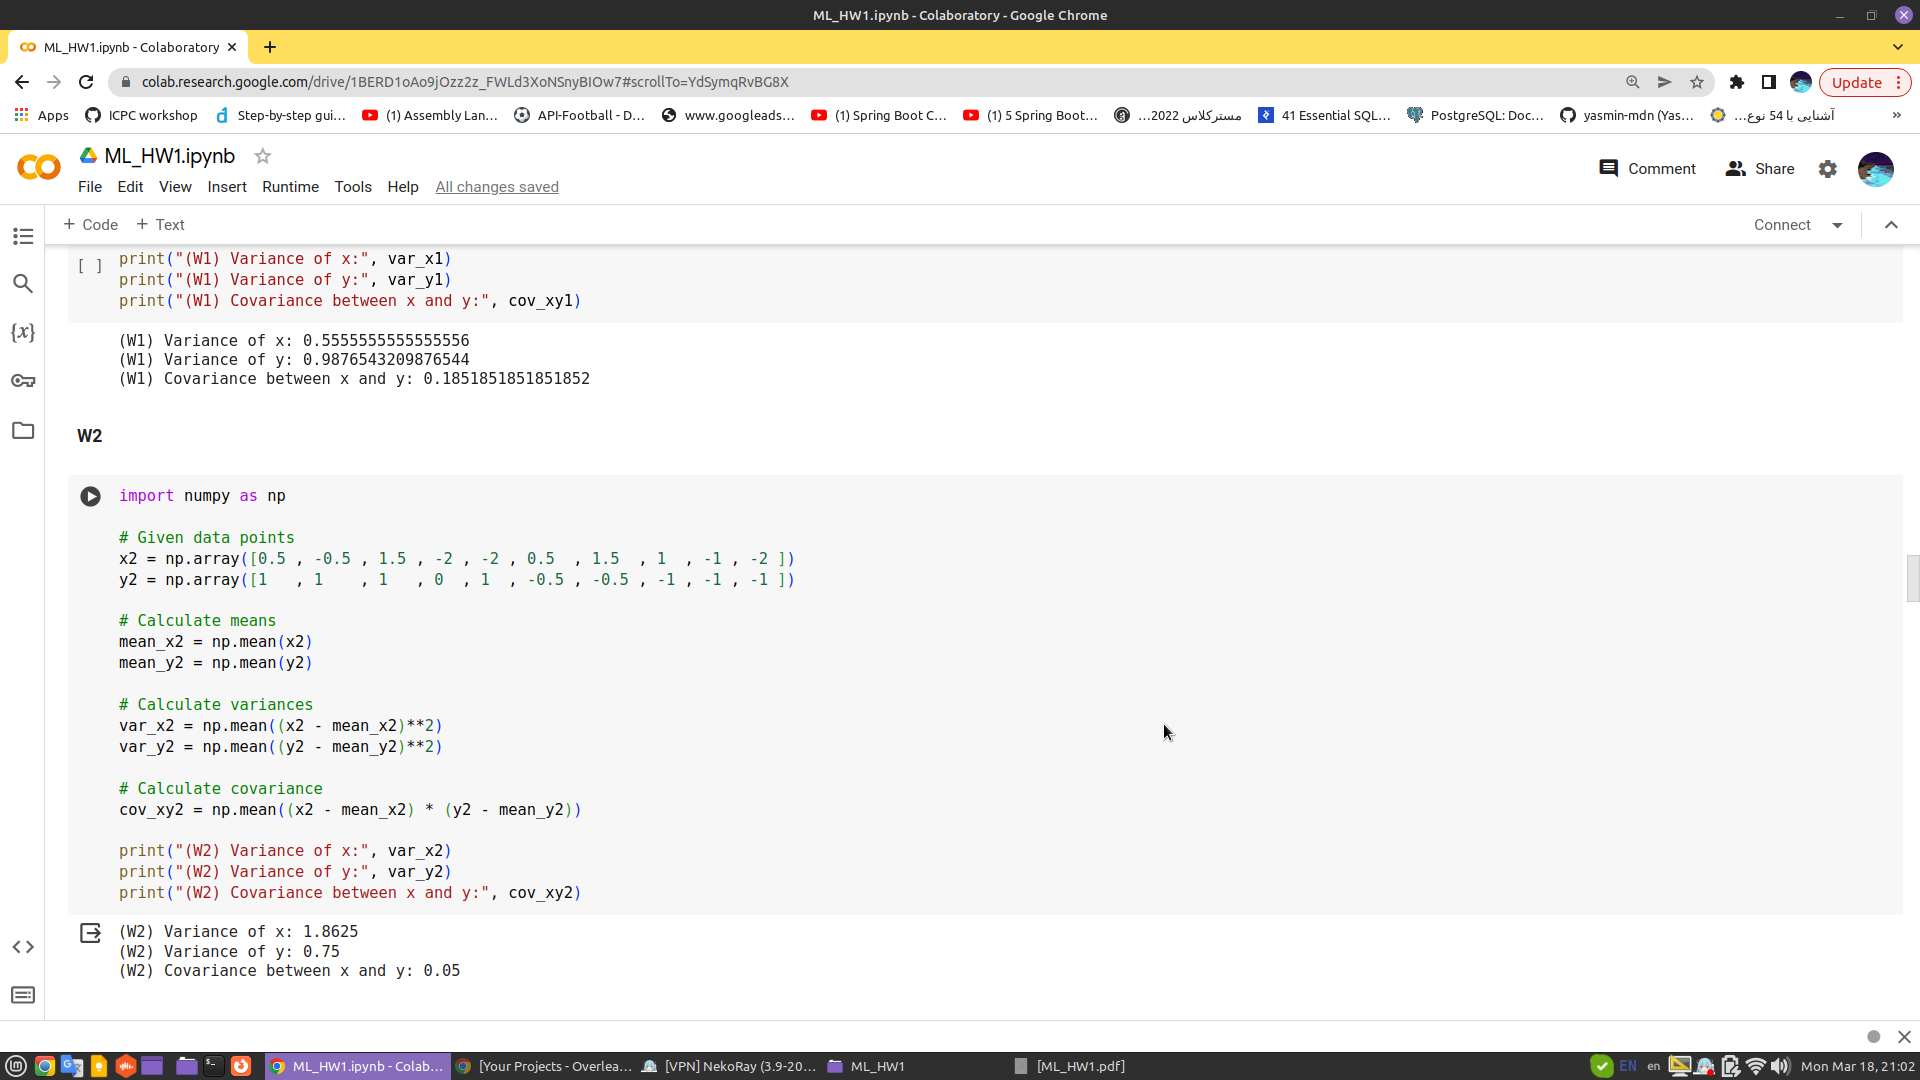
\includegraphics
    [width = 0.8\textwidth]
    {ML1/images/5A.png}
    \caption{محاسبه میانگین و کوواریانس‌ها}
    \label{fig:enter-label}
\end{figure}


\begin{figure}[h]
    \centering
    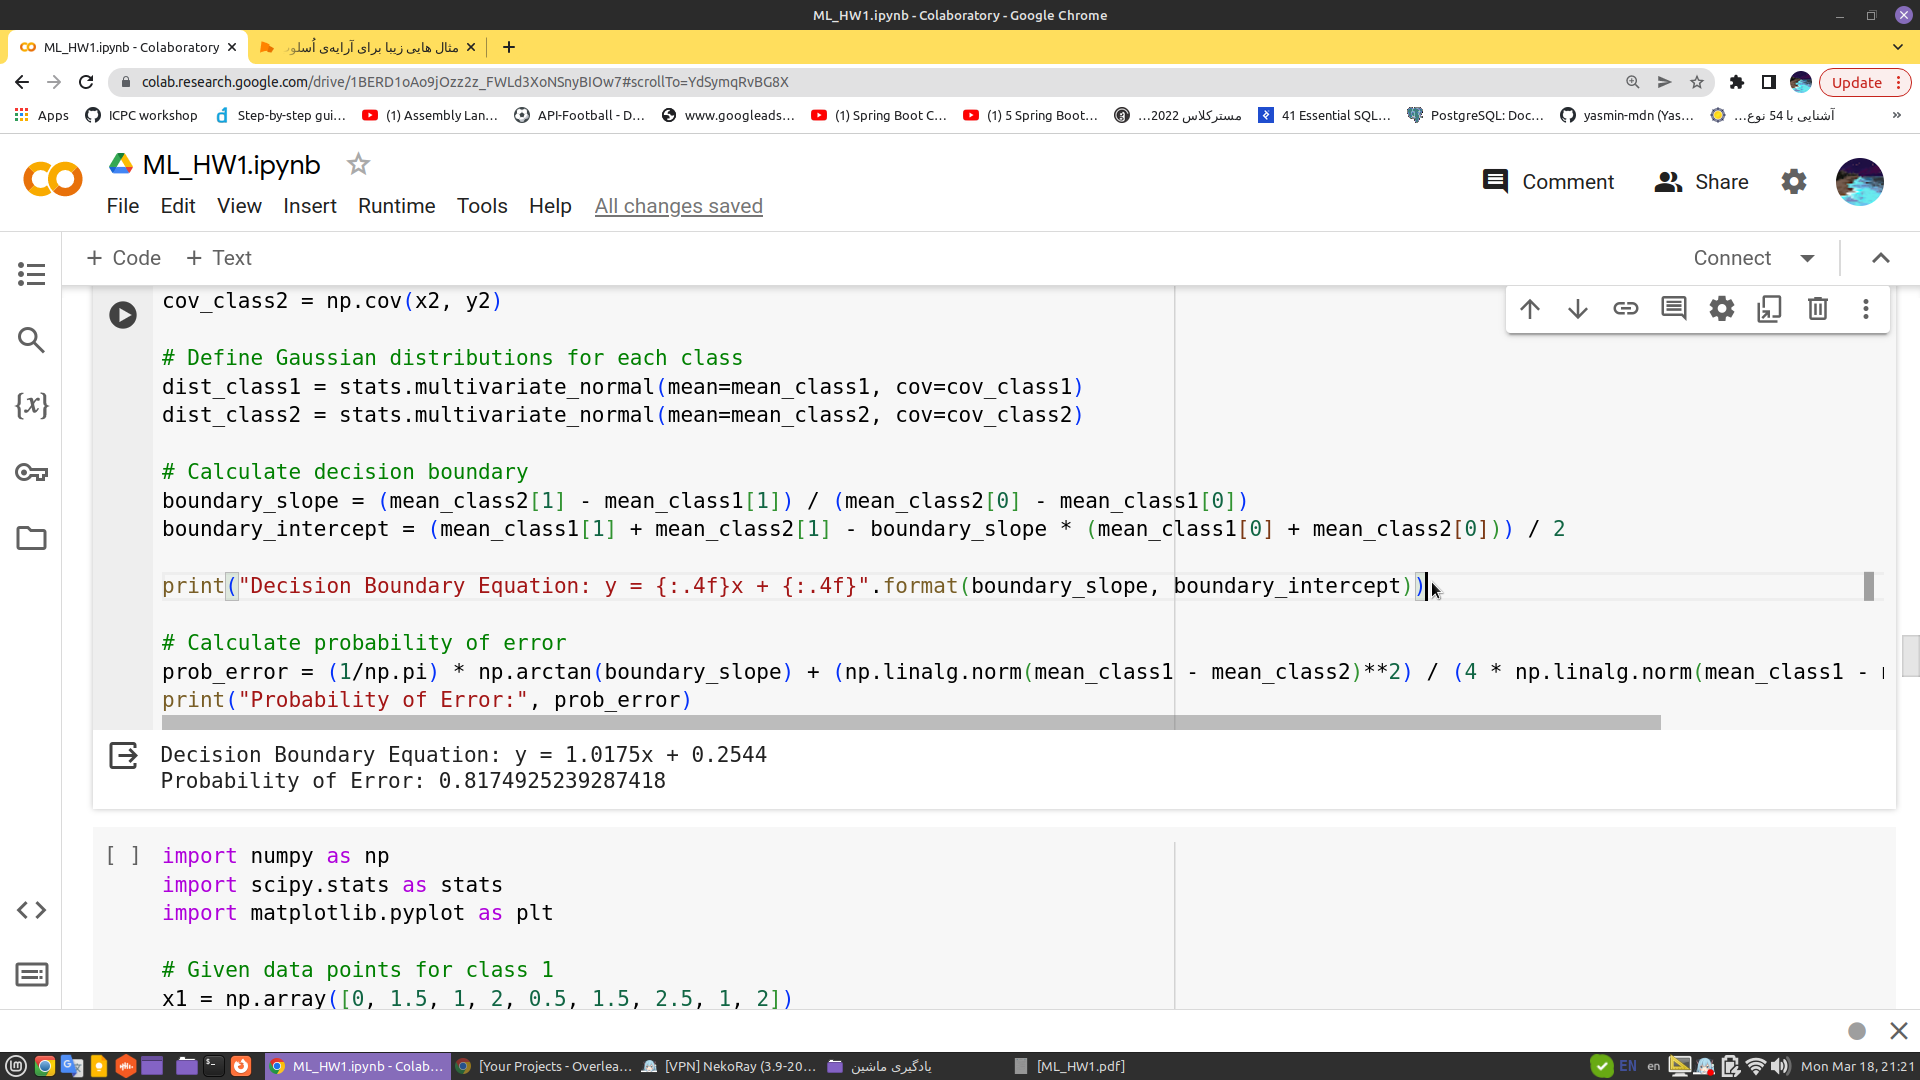
\includegraphics
    [width = 0.8\textwidth]
    {ML1/images/5A2.png}
    \caption{محاسبه میانگین و کوواریانس‌ها}
    \label{fig:enter-label}
\end{figure}

\begin{figure}[h]
    \centering
    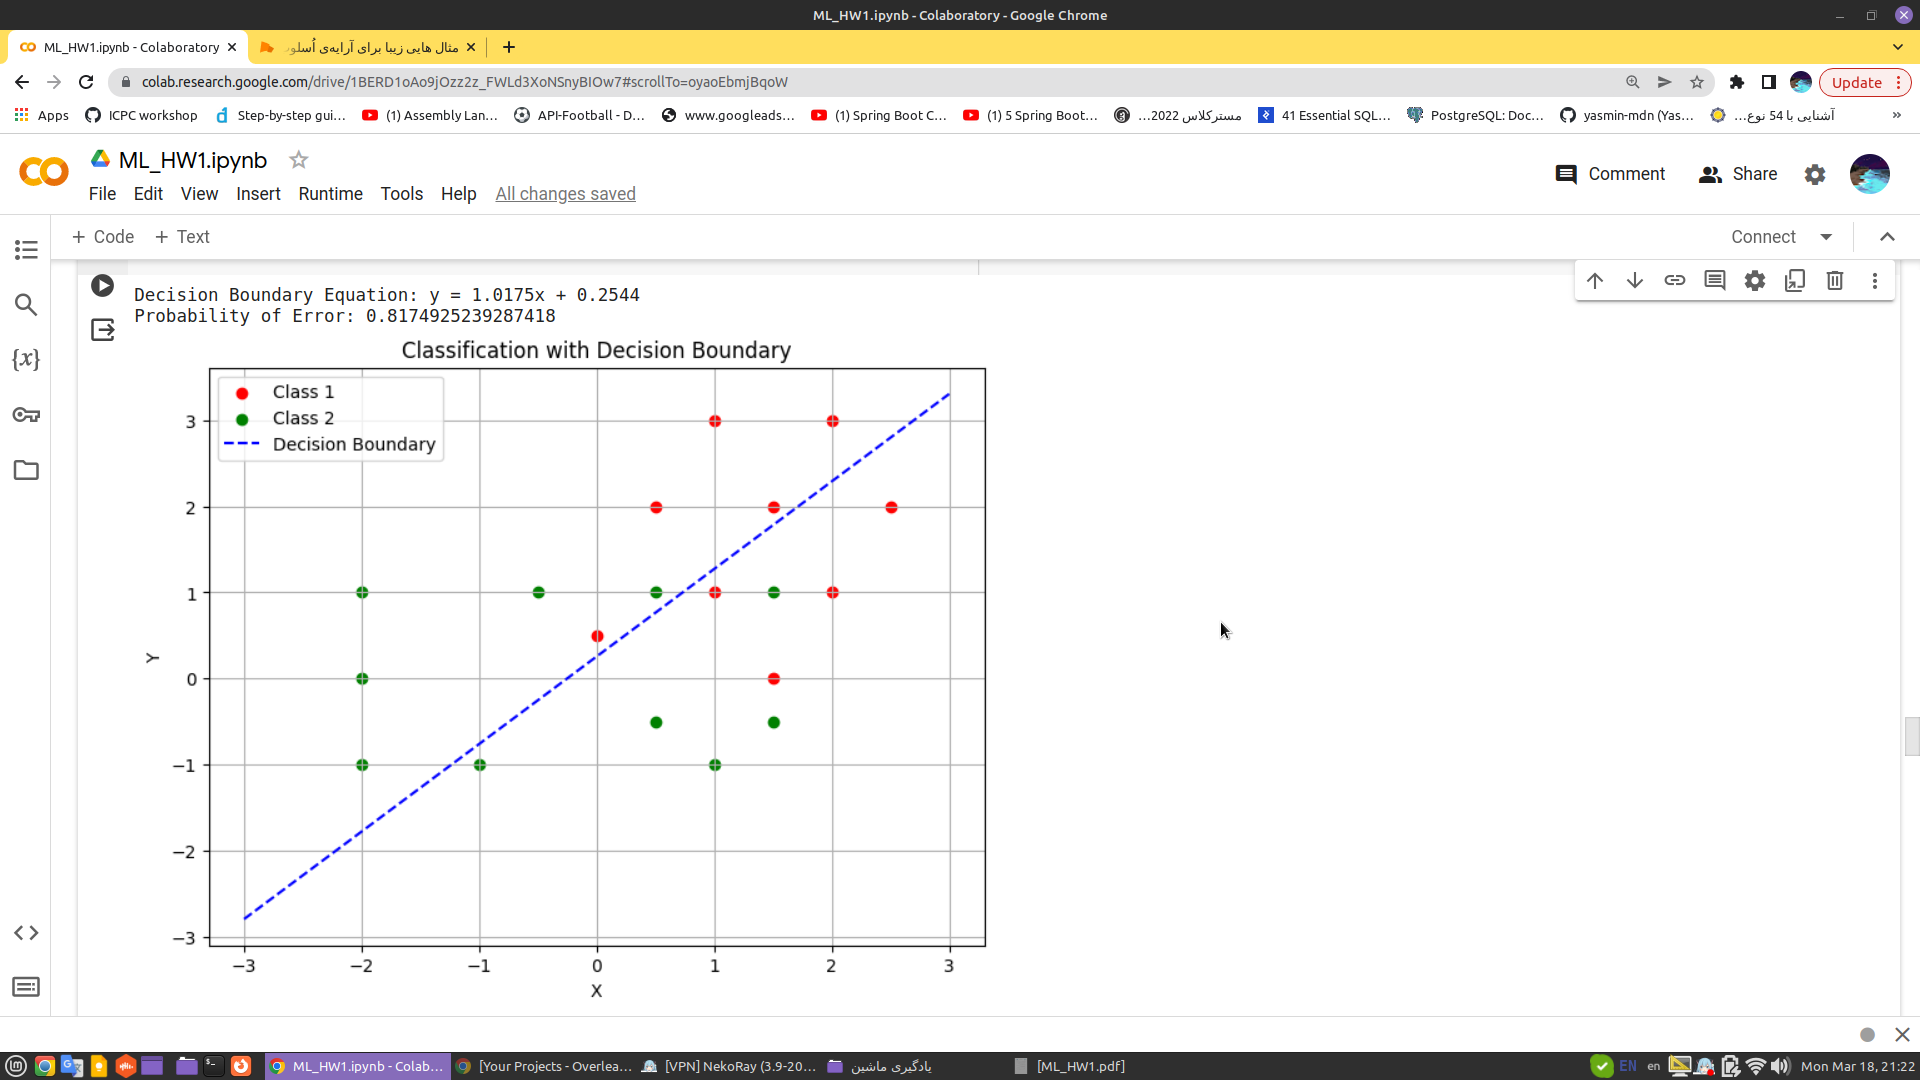
\includegraphics
    [width = 0.8\textwidth]
    {ML1/images/5B.png}
    \caption{محاسبه شیب و عرض‌از‌میدا خط مرز تصمیم}
    \label{fig:enter-label}
\end{figure}

\begin{boxD}
    برای محاسبه خط مرز تصمیم ، شیب و عرض‌از‌مبدا خط واصل بین میانگین دو توزیع گوسی را به‌دست‌خواهیم آورد.
    همانطور که از شکل زیر نیز مشخص‌است تقریبا ۹ نقطه از ۱۹ نقطه به اشتباه طبقه‌بندی شده‌است.
\end{boxD}

\begin{figure}[h]
    \centering
    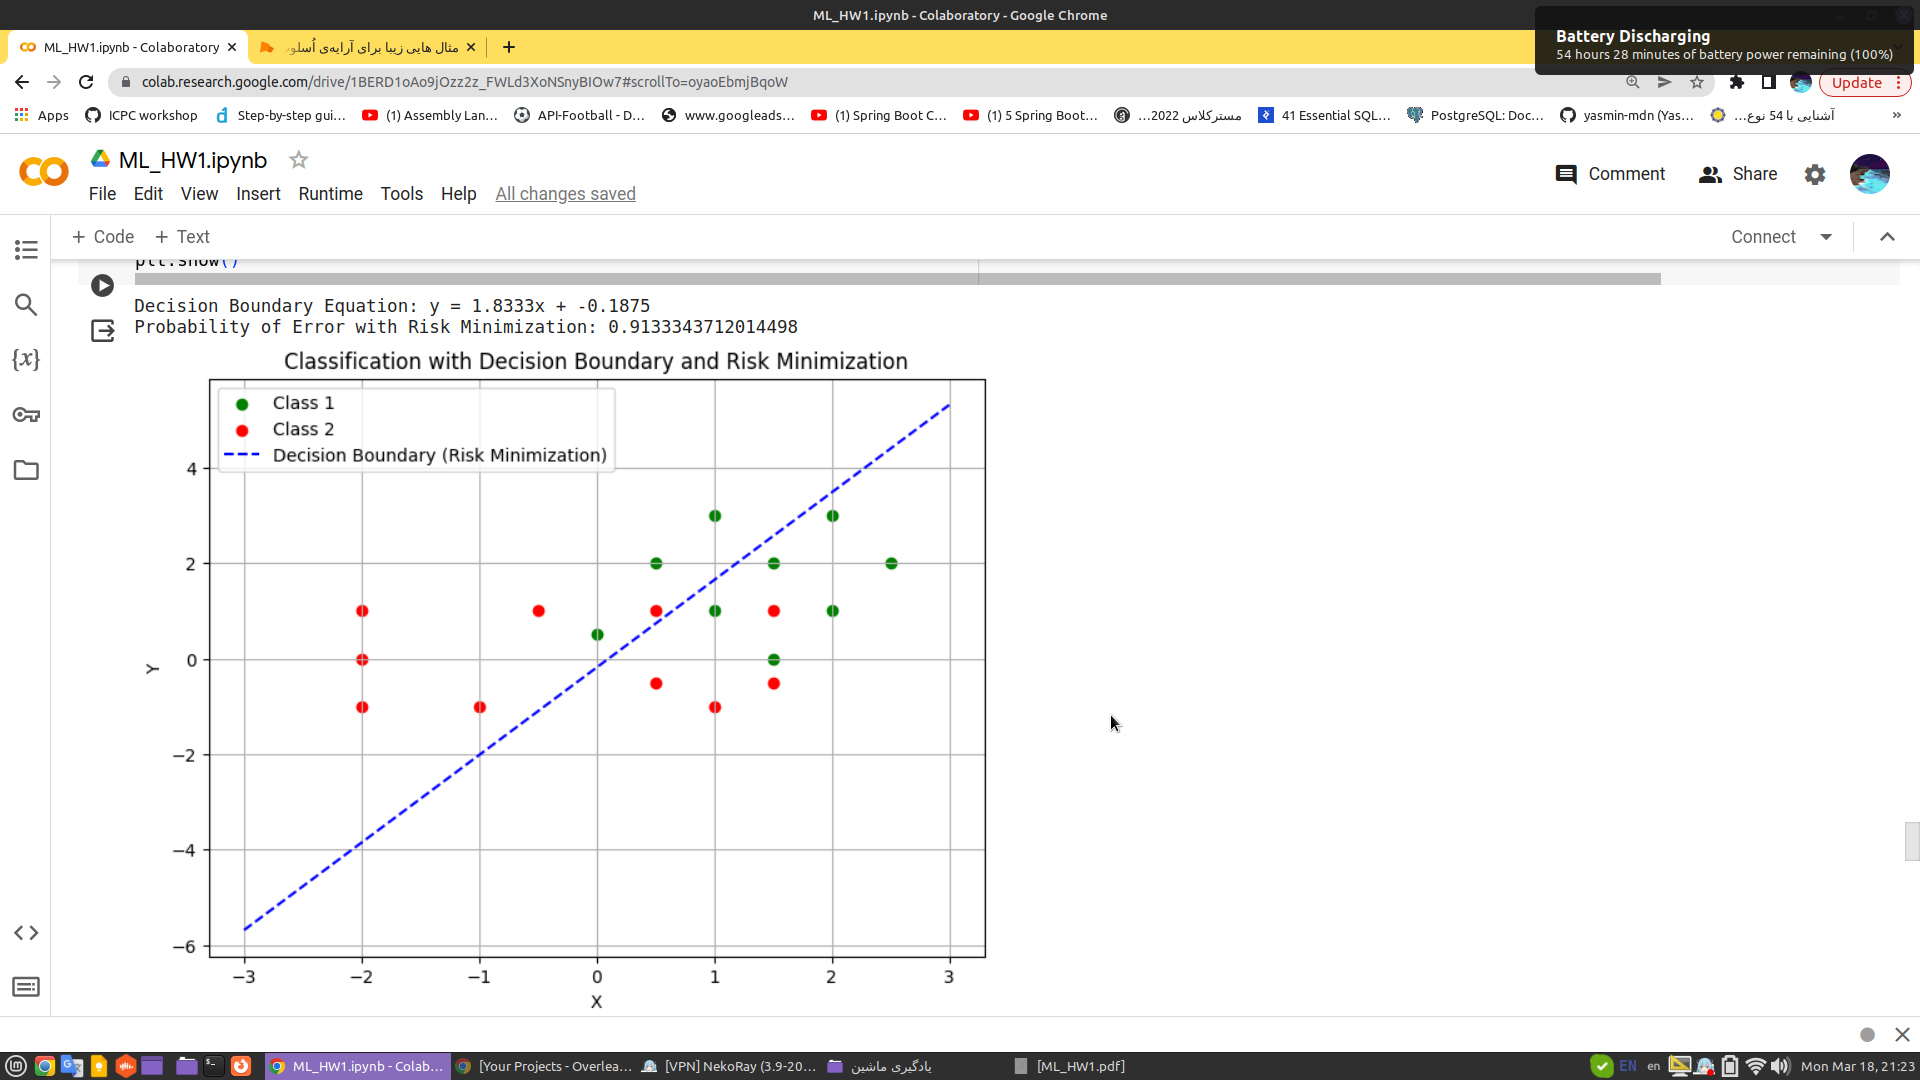
\includegraphics
    [width = 0.8\textwidth]
    {ML1/images/5-P.png}
    \caption{ 
    رسم خط مرز تصمیم
    و ماتریس ریسک
    }
    \label{fig:enter-label}
\end{figure}

\begin{boxD}
    با توجه به مقداردهی هایپرپارامتر ذکرشده در ماتریس ریسک بازهم به محاسبه خط مرز تصمیم و سپس شاهد آن خواهیم‌بود که ۷ نقطه از ۱۹ نقطه به اشتباه طبقه‌بندی شده است.

    متغیری که در تصویر نمایش داده‌شده است در واقع انتگرال مساحت ناحیه خطا می‌باشد.
\end{boxD}

\begin{figure}[h]
    \centering
    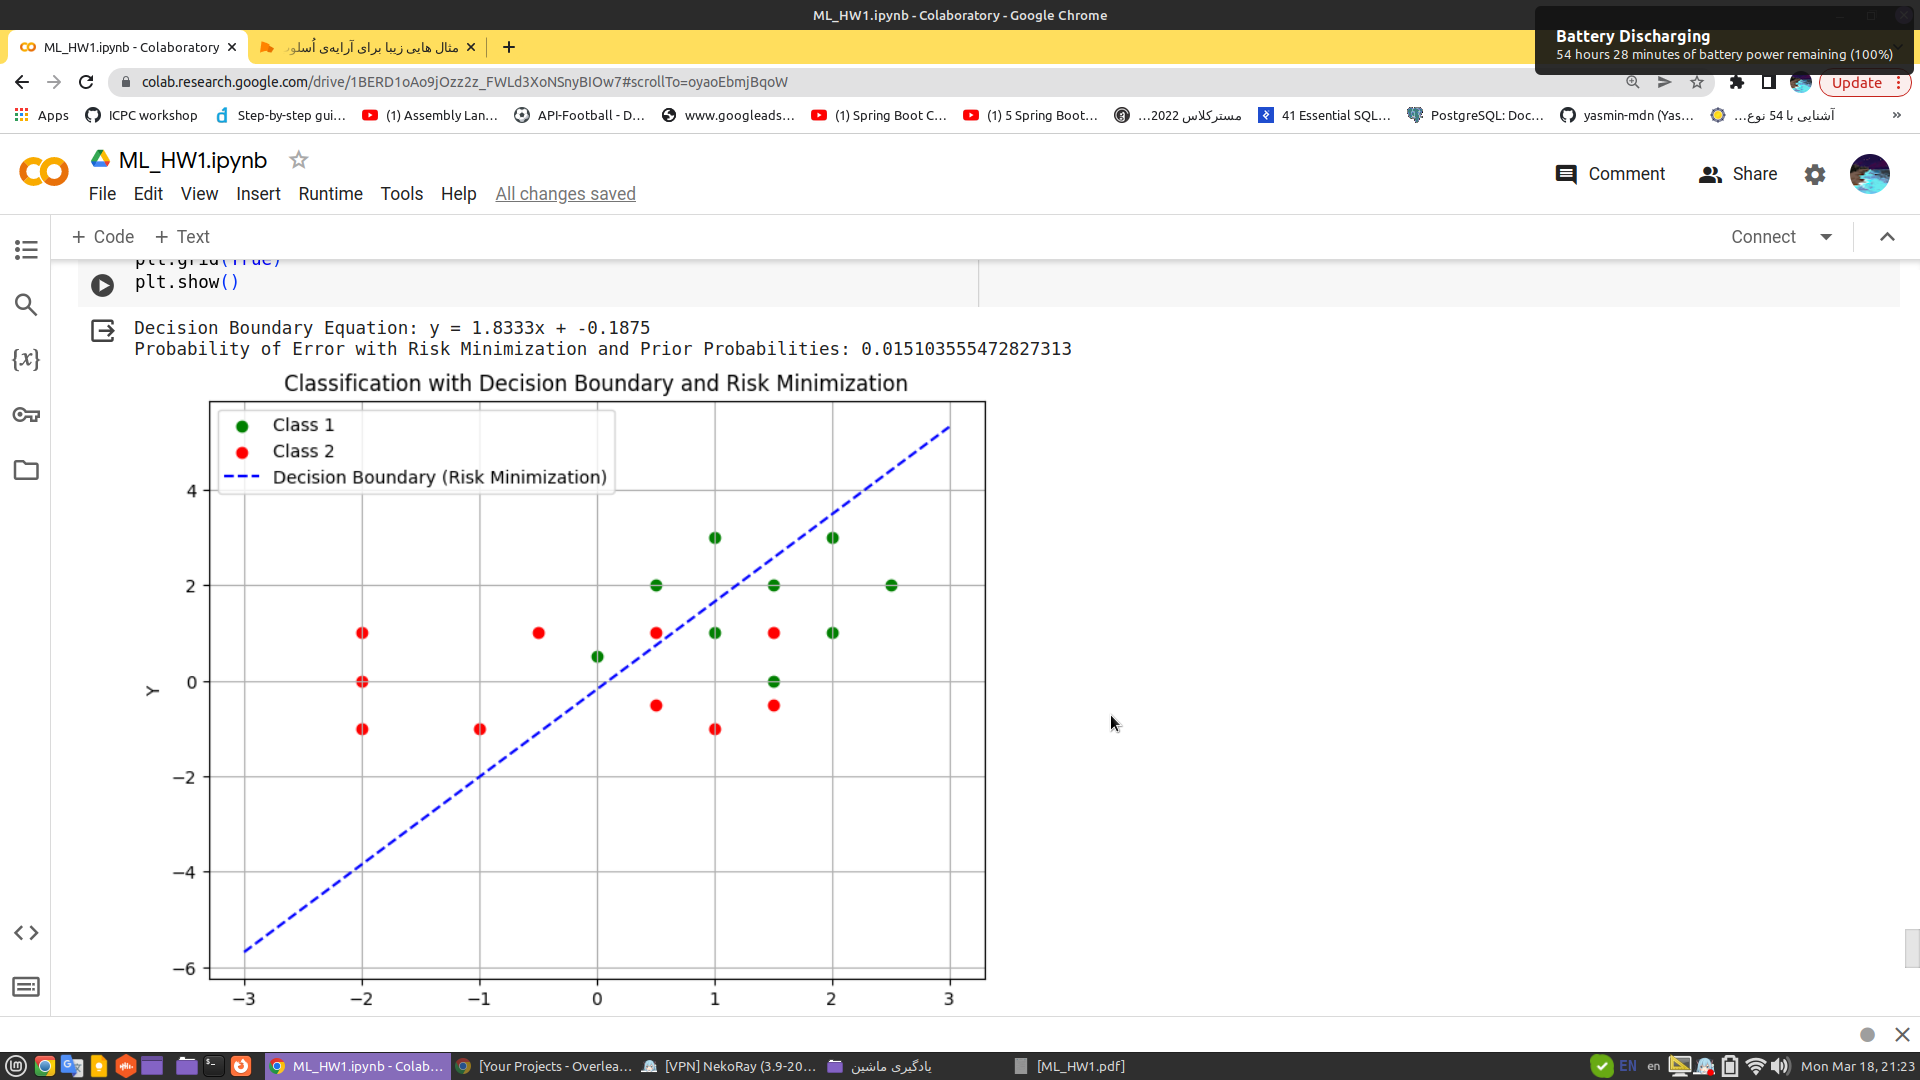
\includegraphics
    [width = 0.8\textwidth]
    {ML1/images/5-T.png}
    \caption{ 
    رسم خط مرز تصمیم با استفاده از ماتریس ریسک
    و احتمال پیشین
    }
    \label{fig:enter-label}
\end{figure}

\begin{boxD}
    نسبت به حالت قبل که از ماتریس ریسک استفاده نکردیم خطا به صورت خوبی کاهش پیدانمود .
\end{boxD}